% ============================================================================
% CHAPTER 3 & 4 CONTENT FROM PART 2
% ============================================================================
% This file contains only the chapter content (no document class or preamble)
% To be imported by OVERLEAF_MASTER_FILE.tex

\chapter{Proposed System}

\section{System Overview}

Salariann is a full-stack web application designed to integrate job discovery, cost-of-living analysis, and personalized career insights into a unified platform. The system architecture comprises four primary layers:

\begin{enumerate}
    \item \textbf{Frontend Layer}: A responsive Flutter web application providing an intuitive user interface for job search, filtering, and career analysis.
    
    \item \textbf{Backend API Layer}: A Node.js/Express server implementing RESTful endpoints for job management, user authentication, and data aggregation.
    
    \item \textbf{AI/ML Services Layer}: Integration points for external APIs (JSearch, Numbeo) and internal algorithms for affordability scoring and recommendation generation.
    
    \item \textbf{Data Persistence Layer}: A Supabase PostgreSQL database storing user profiles, job listings, cost-of-living data, and user interactions.
\end{enumerate}

\begin{figure}[H]
\centering
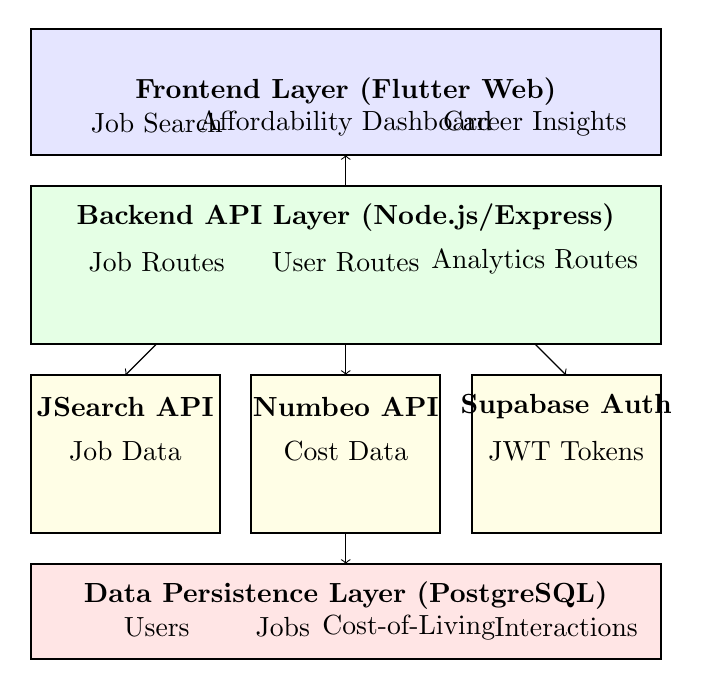
\begin{tikzpicture}[scale=0.8]
    \draw[thick, fill=blue!10] (0,8) rectangle (10,10);
    \node at (5,9) {\textbf{Frontend Layer (Flutter Web)}};
    \node at (2,8.5) {Job Search};
    \node at (5,8.5) {Affordability Dashboard};
    \node at (8,8.5) {Career Insights};
    
    \draw[thick, fill=green!10] (0,5) rectangle (10,7.5);
    \node at (5,7) {\textbf{Backend API Layer (Node.js/Express)}};
    \node at (2,6.3) {Job Routes};
    \node at (5,6.3) {User Routes};
    \node at (8,6.3) {Analytics Routes};
    
    \draw[thick, fill=yellow!10] (0,2) rectangle (3,4.5);
    \node at (1.5,4) {\textbf{JSearch API}};
    \node at (1.5,3.3) {Job Data};
    
    \draw[thick, fill=yellow!10] (3.5,2) rectangle (6.5,4.5);
    \node at (5,4) {\textbf{Numbeo API}};
    \node at (5,3.3) {Cost Data};
    
    \draw[thick, fill=yellow!10] (7,2) rectangle (10,4.5);
    \node at (8.5,4) {\textbf{Supabase Auth}};
    \node at (8.5,3.3) {JWT Tokens};
    
    \draw[thick, fill=red!10] (0,0) rectangle (10,1.5);
    \node at (5,1) {\textbf{Data Persistence Layer (PostgreSQL)}};
    \node at (2,0.5) {Users};
    \node at (4,0.5) {Jobs};
    \node at (6,0.5) {Cost-of-Living};
    \node at (8.5,0.5) {Interactions};
    
    \draw[->] (5,7.5) -- (5,8);
    \draw[->] (2,5) -- (1.5,4.5);
    \draw[->] (5,5) -- (5,4.5);
    \draw[->] (8,5) -- (8.5,4.5);
    \draw[->] (5,2) -- (5,1.5);
\end{tikzpicture}
\caption{High-Level System Architecture Overview}
\label{fig:architecture}
\end{figure}

\section{System Components}

\subsection{Job Discovery Module}

The Job Discovery Module aggregates real-time job listings from multiple sources, normalizes heterogeneous data formats, and exposes a unified job catalog through RESTful endpoints.

\textbf{Responsibilities:}
\begin{itemize}
    \item Fetch live job listings from the JSearch API based on user search queries, location filters, and company preferences.
    \item Transform raw API responses into a standardized internal job schema, ensuring consistent field mapping across sources.
    \item Implement pagination and caching strategies to optimize API usage and reduce latency.
    \item Provide filtering and sorting capabilities on job attributes (role, company, salary range, tech stack, posting date).
\end{itemize}

\subsection{Affordability Analysis Module}

The Affordability Analysis Module integrates real-time cost-of-living data with salary information to produce personalized affordability scores.

\textbf{Responsibilities:}
\begin{itemize}
    \item Scrape current cost-of-living data from Numbeo for supported Indian cities, extracting rent, grocery, transportation, and utility costs.
    \item Implement an in-memory cache with configurable TTL (Time-To-Live) to minimize redundant API calls while maintaining data freshness.
    \item Calculate city-specific expense profiles based on user lifestyle preferences (single vs. family, urban vs. suburban).
    \item Compute affordability scores using a proprietary formula that correlates salary with cost of living.
\end{itemize}

\textbf{Affordability Score Formula:}

Let:
\begin{align*}
S &= \text{Annual salary (in INR)} \\
C &= \text{Annual cost of living (in INR)} \\
D &= \text{Disposable income} = S - C \\
T &= \text{Target disposable income threshold (user-defined, default ₹10 lakhs/year)}
\end{align*}

\begin{equation}
\text{Affordability Score} = \min\left(100, \frac{D}{T} \times 100\right)
\end{equation}

This formula yields a score from 0-100, where 100 represents excellent affordability and 0 represents poor affordability.

\subsection{Career Insights Module}

The Career Insights Module correlates job offers with user preferences, salary trends, and company reputation to generate personalized recommendations and career trajectory projections.

\subsection{User Management and Authentication Module}

The User Management Module handles user registration, authentication, profile management, and personalization preferences.

\section{AI Integration and Data Flow}

\subsection{Automated Data Alignment}

The system automatically aligns heterogeneous job data from multiple sources (JSearch API, internal database) into a unified schema.

\subsection{Affordability-Driven Ranking}

Rather than ranking jobs by recency or popularity, Salariann ranks results by affordability score, ensuring that the most financially viable opportunities appear first.

\subsection{Iterative Recommendation Refinement}

The system implements a feedback loop where user interactions are collected and used to refine recommendation models.

\section{Detailed Workflow of the System}

The following numbered steps trace a complete user journey from initial login through job discovery:

\begin{enumerate}
    \item \textbf{User Authentication}: The user navigates to the Salariann home page and signs in using email and password.
    
    \item \textbf{Profile Setup}: On first login, the user completes a profile questionnaire specifying lifestyle preferences.
    
    \item \textbf{Job Search Initiation}: The user enters a search query and selects one or more cities.
    
    \item \textbf{Real-Time Job Aggregation}: The backend receives the request and calls the JSearch API.
    
    \item \textbf{Data Transformation}: The backend transforms raw JSearch responses into the internal job schema.
    
    \item \textbf{Cost-of-Living Lookup}: For each job's city, the backend checks the in-memory cache for current cost-of-living data.
    
    \item \textbf{Affordability Scoring}: The backend computes an affordability score for each job.
    
    \item \textbf{Response Formatting}: The backend returns a JSON response containing the sorted job list.
    
    \item \textbf{Job Selection and Details}: The user clicks on a job card to view full details.
    
    \item \textbf{Application or Save}: The user either applies for the job or saves the job for later review.
\end{enumerate}

% ============================================================================
% CHAPTER 4: SYSTEM DESIGN
% ============================================================================
\chapter{System Design}

\section{System Architecture Diagram}

\begin{figure}[H]
\centering
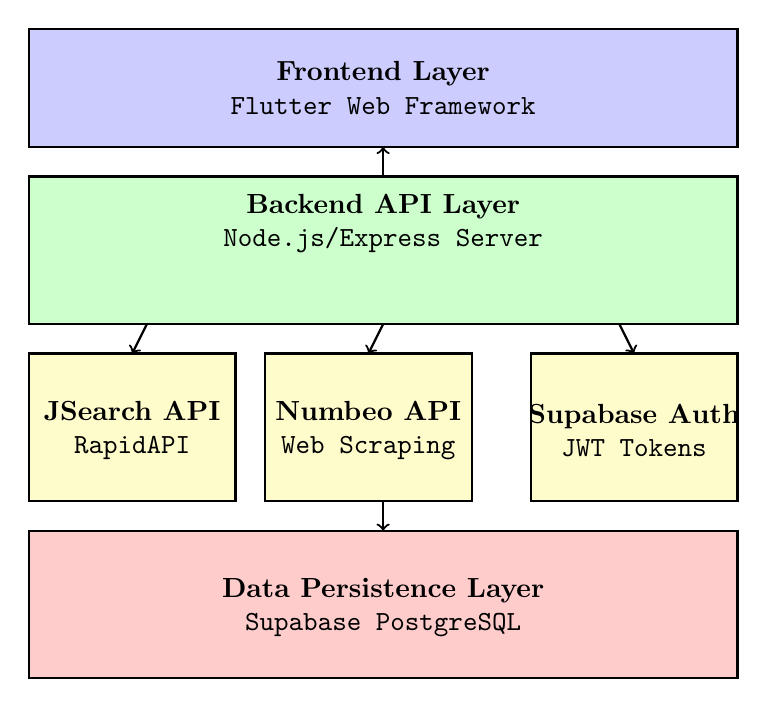
\begin{tikzpicture}[scale=0.75]
    \draw[thick, fill=blue!20] (0,10) rectangle (12,12);
    \node[align=center] at (6,11) {\textbf{Frontend Layer}\\\texttt{Flutter Web Framework}};
    
    \draw[thick, fill=green!20] (0,7) rectangle (12,9.5);
    \node[align=center] at (6,8.7) {\textbf{Backend API Layer}\\\texttt{Node.js/Express Server}};
    
    \draw[thick, fill=yellow!20] (0,4) rectangle (3.5,6.5);
    \node[align=center] at (1.75,5.2) {\textbf{JSearch API}\\\texttt{RapidAPI}};
    
    \draw[thick, fill=yellow!20] (4,4) rectangle (7.5,6.5);
    \node[align=center] at (5.75,5.2) {\textbf{Numbeo API}\\\texttt{Web Scraping}};
    
    \draw[thick, fill=yellow!20] (8.5,4) rectangle (12,6.5);
    \node[align=center] at (10.25,5.2) {\textbf{Supabase Auth}\\\texttt{JWT Tokens}};
    
    \draw[thick, fill=red!20] (0,1) rectangle (12,3.5);
    \node[align=center] at (6,2.2) {\textbf{Data Persistence Layer}\\\texttt{Supabase PostgreSQL}};
    
    \draw[->, thick] (6,9.5) -- (6,10);
    \draw[->, thick] (2,7) -- (1.75,6.5);
    \draw[->, thick] (6,7) -- (5.75,6.5);
    \draw[->, thick] (10,7) -- (10.25,6.5);
    \draw[->, thick] (6,4) -- (6,3.5);
\end{tikzpicture}
\caption{Detailed System Architecture Diagram}
\label{fig:detailed_arch}
\end{figure}

\section{Data Flow Diagram}

\subsection{Level 0 Context Diagram}

\begin{figure}[H]
\centering
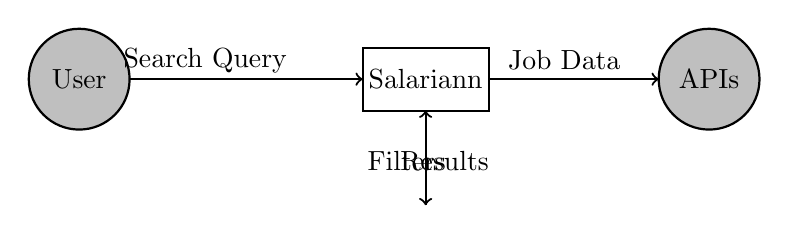
\begin{tikzpicture}[scale=0.8]
    \draw[circle, thick, fill=lightgray] (1,5) circle (0.8);
    \node at (1,5) {User};
    
    \draw[circle, thick, fill=lightgray] (11,5) circle (0.8);
    \node at (11,5) {APIs};
    
    \draw[thick, fill=white] (5.5,4.5) rectangle (7.5,5.5);
    \node at (6.5,5) {Salariann};
    
    \draw[->, thick] (1.8,5) -- (5.5,5);
    \node at (3,5.3) {Search Query};
    
    \draw[->, thick] (7.5,5) -- (10.2,5);
    \node at (8.7,5.3) {Job Data};
    
    \draw[->, thick] (6.5,4.5) -- (6.5,3);
    \node at (6.8,3.7) {Results};
    
    \draw[->, thick] (6.5,3) -- (6.5,4.5);
    \node at (6.2,3.7) {Filters};
\end{tikzpicture}
\caption{Context Diagram (Level 0 DFD)}
\label{fig:dfd_l0}
\end{figure}

\subsection{Level 1 Detailed Data Flow Diagram}

\begin{figure}[H]
\centering
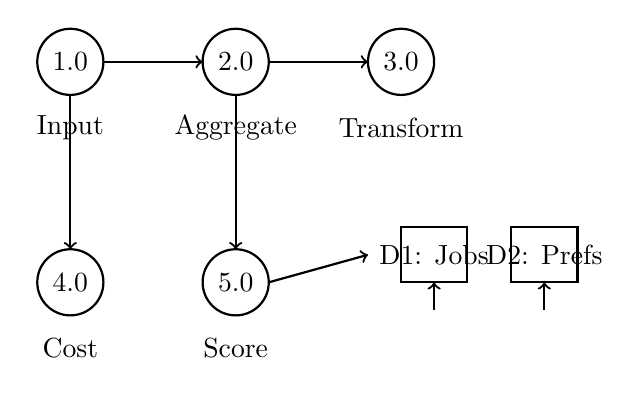
\begin{tikzpicture}[scale=0.7]
    \draw[circle, thick] (2,8) circle (0.6);
    \node at (2,8) {1.0};
    \node at (2,6.8) {Input};
    
    \draw[circle, thick] (5,8) circle (0.6);
    \node at (5,8) {2.0};
    \node at (5,6.8) {Aggregate};
    
    \draw[circle, thick] (8,8) circle (0.6);
    \node at (8,8) {3.0};
    \node at (8,6.8) {Transform};
    
    \draw[circle, thick] (2,4) circle (0.6);
    \node at (2,4) {4.0};
    \node at (2,2.8) {Cost};
    
    \draw[circle, thick] (5,4) circle (0.6);
    \node at (5,4) {5.0};
    \node at (5,2.8) {Score};
    
    \draw[rectangle, thick] (8,4) rectangle (9.2,5);
    \node at (8.6,4.5) {D1: Jobs};
    
    \draw[rectangle, thick] (10,4) rectangle (11.2,5);
    \node at (10.6,4.5) {D2: Prefs};
    
    \draw[->, thick] (2.6,8) -- (4.4,8);
    \draw[->, thick] (5.6,8) -- (7.4,8);
    \draw[->, thick] (2,7.4) -- (2,4.6);
    \draw[->, thick] (5,7.4) -- (5,4.6);
    \draw[->, thick] (5.6,4) -- (7.4,4.5);
    \draw[->, thick] (8.6,3.5) -- (8.6,4);
    \draw[->, thick] (10.6,3.5) -- (10.6,4);
\end{tikzpicture}
\caption{Detailed Data Flow Diagram (Level 1 DFD)}
\label{fig:dfd_l1}
\end{figure}

\section{UML Diagrams}

\subsection{Use Case Diagram}

\begin{figure}[H]
\centering
\begin{tikzpicture}[scale=0.8]
    \draw[thick, rectangle] (2,1) rectangle (8,7);
    \node at (5,6.7) {Salariann System};
    
    \draw[ellipse, thick] (3.5,5.5) ellipse (1,0.5);
    \node at (3.5,5.5) {Search Jobs};
    
    \draw[ellipse, thick] (5,5.5) ellipse (1,0.5);
    \node at (5,5.5) {View Details};
    
    \draw[ellipse, thick] (6.5,5.5) ellipse (1,0.5);
    \node at (6.5,5.5) {Save Job};
    
    \draw[ellipse, thick] (4,3.5) ellipse (1,0.5);
    \node at (4,3.5) {Calculate};
    
    \draw[ellipse, thick] (6,3.5) ellipse (1,0.5);
    \node at (6,3.5) {View Insights};
    
    \draw[circle, thick, fill=lightgray] (0.5,4) circle (0.5);
    \node at (0.5,4) {User};
    
    \draw[circle, thick, fill=lightgray] (9,4) circle (0.5);
    \node at (9,4) {APIs};
    
    \draw[-] (1,4) -- (2,5.5);
    \draw[-] (1,4) -- (2,3.5);
    \draw[-] (8,4) -- (8,5.5);
\end{tikzpicture}
\caption{Use Case Diagram}
\label{fig:usecase}
\end{figure}

\subsection{Class Diagram}

\begin{table}[H]
\centering
\caption{Key Classes and Their Responsibilities}
\label{tab:classes}
\begin{tabular}{|l|l|l|}
\hline
\textbf{Class} & \textbf{Key Attributes} & \textbf{Key Methods} \\
\hline
User & id, email, displayName, lifestyle & signUp(), login(), updateProfile() \\
\hline
Job & id, title, company, salary, city & getDetails(), calculateScore() \\
\hline
Company & id, name, logoUrl, website & getProfile(), getReviews() \\
\hline
CostOfLiving & id, city, rent, grocery, transport & getProfile(), updateData() \\
\hline
AffordabilityScore & jobId, userId, score & calculate(), getBreakdown() \\
\hline
\end{tabular}
\end{table}

\section{Database Schema}

\begin{table}[H]
\centering
\caption{Database Schema and Storage Strategy}
\label{tab:schema}
\begin{tabular}{|l|l|p{6cm}|}
\hline
\textbf{Table} & \textbf{Type} & \textbf{Description} \\
\hline
users & PostgreSQL & User profiles with authentication data \\
\hline
jobs & PostgreSQL & Job listings from JSearch and local sources \\
\hline
companies & PostgreSQL & Company information and metadata \\
\hline
cost\_of\_living & PostgreSQL & City-specific cost-of-living data \\
\hline
user\_job\_interactions & PostgreSQL & User behavior tracking and analytics \\
\hline
reviews & PostgreSQL & User-submitted company reviews \\
\hline
\end{tabular}
\end{table}

\section{Entity Relationship Diagram}

\begin{figure}[H]
\centering
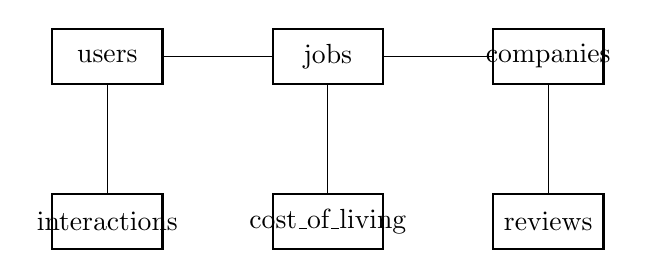
\begin{tikzpicture}[scale=0.7]
    \draw[rectangle, thick] (1,8) rectangle (3,9);
    \node at (2,8.5) {users};
    
    \draw[rectangle, thick] (5,8) rectangle (7,9);
    \node at (6,8.5) {jobs};
    
    \draw[rectangle, thick] (9,8) rectangle (11,9);
    \node at (10,8.5) {companies};
    
    \draw[rectangle, thick] (5,5) rectangle (7,6);
    \node at (6,5.5) {cost\_of\_living};
    
    \draw[rectangle, thick] (1,5) rectangle (3,6);
    \node at (2,5.5) {interactions};
    
    \draw[rectangle, thick] (9,5) rectangle (11,6);
    \node at (10,5.5) {reviews};
    
    \draw[-] (3,8.5) -- (5,8.5);
    \draw[-] (7,8.5) -- (9,8.5);
    \draw[-] (6,8) -- (6,6);
    \draw[-] (2,8) -- (2,6);
    \draw[-] (10,8) -- (10,6);
    \draw[-] (6,5) -- (6,5);
\end{tikzpicture}
\caption{Entity Relationship Diagram}
\label{fig:erd}
\end{figure}
